\section{Analysis}
\subsection{Processed Data}
In order to derive the relationship in the data, I first determined the average resistance. To calculate the absolute and percent average uncertainty for the resistances, the following formulas can be applied. Sample calculations for $T=20^\circ C$ are shown below.
\[\delta R_{avg}=\frac{R_{max}-R_{min}}{2\sqrt{N}}=\frac{20.00\;k\Omega -14.40\;k\Omega}{2\sqrt{5}}=1.25\;k\Omega\]

\[\frac{\delta R_{avg}}{R_{avg}}=\frac{1.25\;k\Omega}{17.12\;k\Omega}=7.31\%\]

\begin{longtable}{| >{\centering\arraybackslash}p{0.17\linewidth} | >{\centering\arraybackslash}p{0.15\linewidth} | >{\centering\arraybackslash}p{0.25\linewidth} | >{\centering\arraybackslash}p{0.25\linewidth} |}
\hline
    Temperature (± 0.1 °C) & Average Resistance ($k\Omega$) & Average Resistance Uncertainty ($k\Omega$) & Average Resistance Uncertainty (\%) \\ \hline
    20.0 & 17.12 & 1.25 & 7.31 \\ \hline
    25.0 & 14.07 & 0.92 & 6.55 \\ \hline
    30.0 & 12.00 & 0.83 & 6.95 \\ \hline
    35.0 & 10.13 & 0.59 & 5.87 \\ \hline
    40.0 & 8.59 & 0.42 & 4.84 \\ \hline
    45.0 & 7.28 & 0.36 & 4.92 \\ \hline
    50.0 & 6.27 & 0.22 & 3.57 \\ \hline
    55.0 & 5.13 & 0.17 & 3.36 \\ \hline
    60.0 & 4.37 & 0.18 & 4.14 \\ \hline
    65.0 & 3.71 & 0.10 & 2.65 \\ \hline
    70.0 & 3.16 & 0.08 & 2.61 \\ \hline
    75.0 & 2.65 & 0.08 & 3.21 \\ \hline
    80.0 & 2.27 & 0.06 & 2.66 \\ \hline
    85.0 & 1.93 & 0.04 & 1.96 \\ \hline
    90.0 & 1.67 & 0.04 & 2.26 \\ \hline
    95.0 & 1.49 & 0.02 & 1.20 \\ \hline
\caption{Average Resistance of an NTC Thermistor at a given Temperature}
\end{longtable}

\begin{figure}[H]
    \centering
    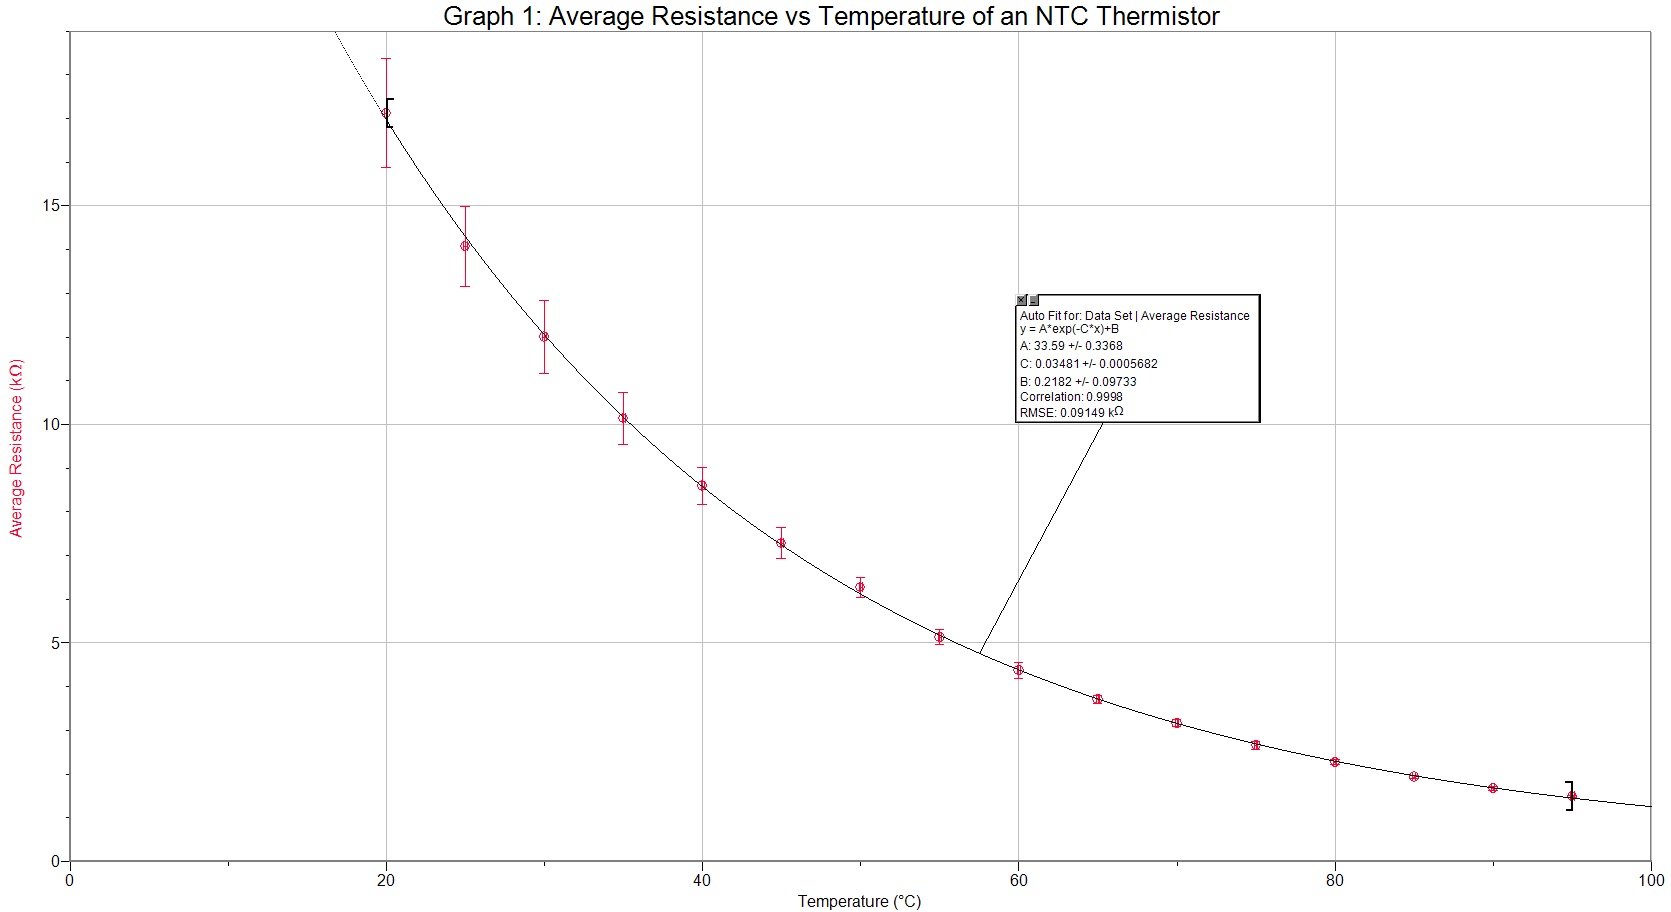
\includegraphics[width=120mm,height=\textheight,keepaspectratio]{images/before_linearization.png}
    \caption{Graph of Average Resistance vs Temperature}
    \label{fig:before_linearization}
\end{figure}

\subsection{Linearization: Beta Model}
Since there is a very strong correlation ($R^2=0.9998$) of the data to an exponential fit (Figure \ref{fig:before_linearization}), the data should be linearized to better perform and interpret the slope. This data can be linearized using the Beta Model for a Thermistor shown below \citep{amethermbetamodel}.
\[\beta=\frac{\ln{\frac{R_2}{R_1}}}{\frac{1}{T_2}-\frac{1}{T_1}}\]
\[\ln{R_{avg}}=\beta\frac{1}{T}+\ln{R_0}\]

Note that the temperature is in Kelvin. Therefore, the following formula must be applied.

\[T_K=T_C+273\;K\]

The uncertainties for $\ln{R_avg}$ and $\frac{1}{T}$ can be determined using the Law of Propagation of Uncertainty \citep{taylor_1982}.
\[\delta f(x,y,\dots)=\sqrt{\left(\frac{\partial f}{\partial x}\delta x \right)^2+ \left(\frac{\partial f}{\partial y}\delta y \right)^2+\dots}\]

Thus, for $\ln{R_{avg}}$:
\[\delta \ln{(R_{avg})}=\sqrt{\left(\frac{\partial \ln{R_{avg}}}{\partial R_{avg}}\delta R_{avg} \right)^2}=\frac{\delta R_{avg}}{R_{avg}}=\frac{1.25\;k\Omega}{17.12\;k\Omega}=0.07 \;\ln{k\Omega}\]

Note that units for the linearized resistance are in $\ln{k\Omega}$, since they have a different dimension than the $k\Omega$.

Similarly, for $\frac{1}{T}$:
\[\delta \frac{1}{T}=\sqrt{\left(\frac{\partial \frac{1}{T}}{\partial x}\delta T \right)^2}=\frac{\delta T}{T^2}=\frac{0.1 K}{(293.0 \; K)^2}=0.000001 \;\frac{1}{K}\]

\begin{longtable}{| >{\centering\arraybackslash}p{0.2\linewidth} | >{\centering\arraybackslash}p{0.25\linewidth} | >{\centering\arraybackslash}p{0.15\linewidth} | >{\centering\arraybackslash}p{0.25\linewidth} |}
\hline
    Reciprocal of Temperature (1/K) & Reciprocal of Temperature Uncertainty (1/K) & ln of Average Resistance ($ln{k\Omega}$) & ln of Average Resistance Uncertainty ($ln{k\Omega}$) \\ \hline
    0.003413 & 0.000001 & 2.84 & 0.07 \\ \hline
    0.003356 & 0.000001 & 2.64 & 0.07 \\ \hline
    0.003300 & 0.000001 & 2.48 & 0.07 \\ \hline
    0.003247 & 0.000001 & 2.32 & 0.06 \\ \hline
    0.003195 & 0.000001 & 2.15 & 0.05 \\ \hline
    0.003145 & 0.000001 & 1.98 & 0.05 \\ \hline
    0.003096 & 0.000001 & 1.84 & 0.04 \\ \hline
    0.003049 & 0.000001 & 1.64 & 0.03 \\ \hline
    0.003003 & 0.000001 & 1.47 & 0.04 \\ \hline
    0.002959 & 0.000001 & 1.31 & 0.03 \\ \hline
    0.002915 & 0.000001 & 1.15 & 0.03 \\ \hline
    0.002874 & 0.000001 & 0.97 & 0.03 \\ \hline
    0.002833 & 0.000001 & 0.82 & 0.03 \\ \hline
    0.002793 & 0.000001 & 0.66 & 0.02 \\ \hline
    0.002755 & 0.000001 & 0.51 & 0.02 \\ \hline
    0.002717 & 0.000001 & 0.40 & 0.01 \\ \hline
    \caption{Natural Log of Average Resistance vs Reciprocal of Temperature of an NTC Thermistor}
\end{longtable}

\begin{figure}[H]
    \centering
    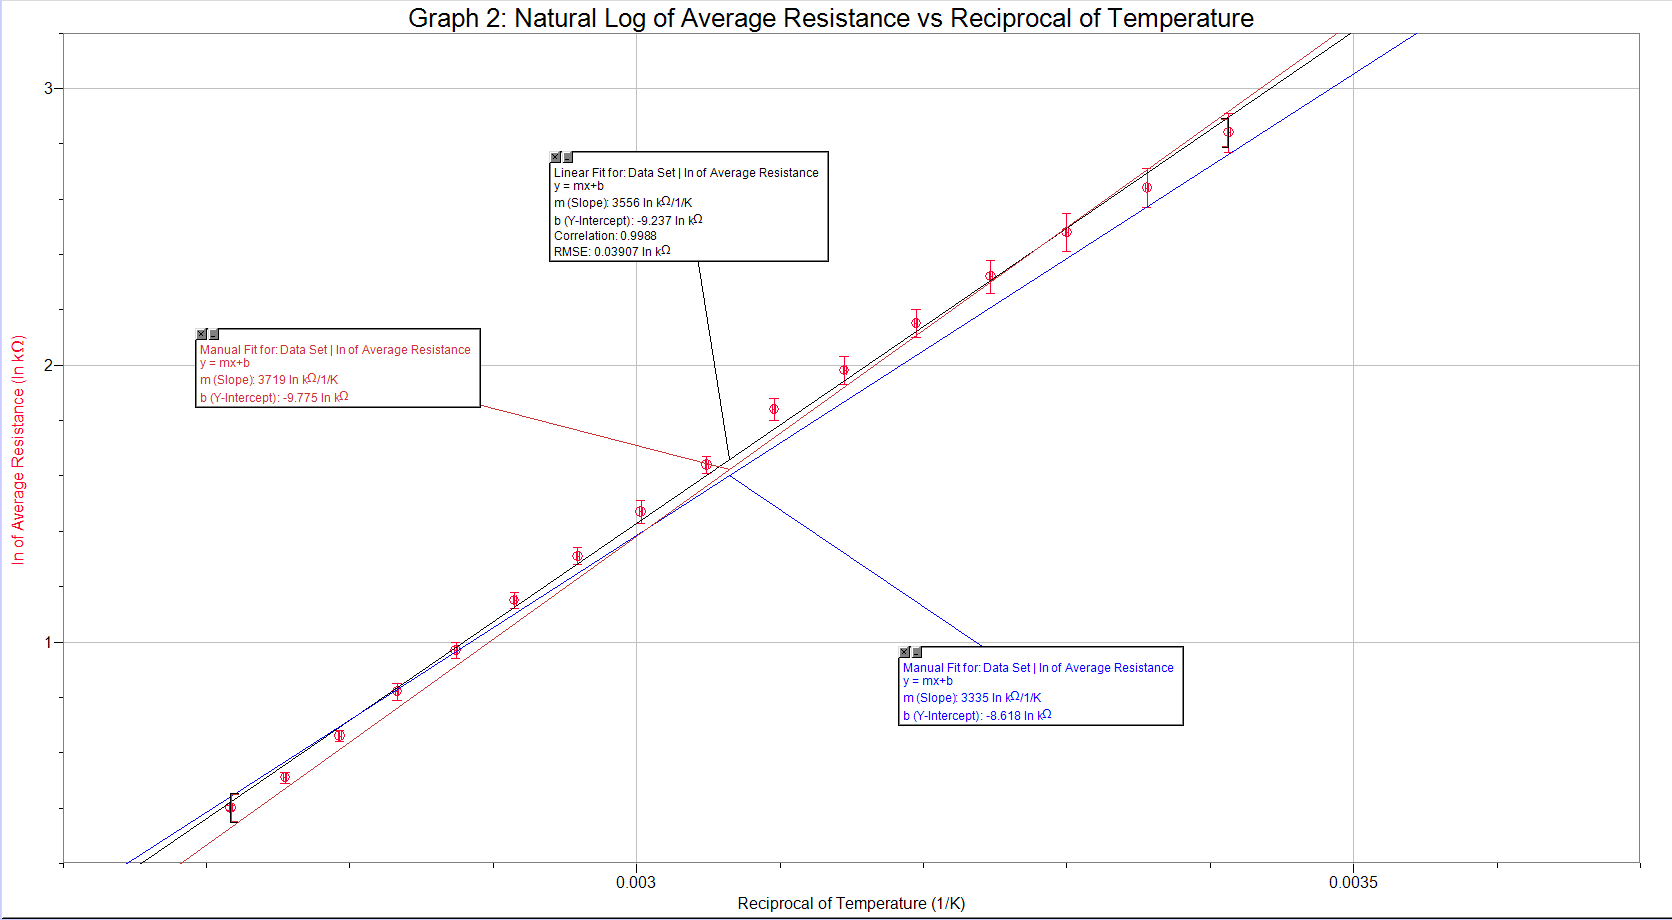
\includegraphics[width=120mm,height=\textheight,keepaspectratio]{images/after_linearization.png}
    \caption{Graph of Natural Log of Average Resistance vs Reciprocal of Temperature}
    \label{fig:after_linearization}
\end{figure}

\subsection{Percent Uncertainty and Percent Error of Slope}
A rough estimate of the percent uncertainty of the slope $\beta$ can be determined by utilizing the maximum and minimum slope lines.
\[\delta \beta = \frac{\beta_{max}-\beta_{min}}{2} = \frac{3719 K \ln{k\Omega}-3335 K \ln{k\Omega}}{2}=192 K \ln{k\Omega}\]
\[\frac{\delta \beta}{\beta}=\frac{192 K \ln{k\Omega}}{3556 K \ln{k\Omega}}=5.40 \%\]

The accepted value for the slope $\beta$ for this NTC Themistor is $3474 K \ln{k\Omega}$.
Therefore, to calculate the percent error, the following calculation can be performed.
\[Percent \; Error = \frac{|\beta_{actual} - \beta_{accepted}|}{\beta_{accepted}}=\frac{|3556 K \ln{k\Omega} - 3474 K \ln{k\Omega}|}{3474 K \ln{k\Omega}}=2.36\%\]


\subsection{Interpretation}
As seen in the Linearized Beta Model Graph (Figure \ref{fig:after_linearization}), the line of best fit indicates a positive linear relationship between $\ln{R}$ and $\frac{1}{T}$. This means as $\frac{1}{T}$ increases, $\ln{R}$ will increase proportionally. Furthermore, this linearization proves that there is a negative exponential relationship between $R$ and $T$.

There is a very strong correlation ($R^2=0.9988$) between the linear regression and the linearized data. The line of best fit passes through almost all points and uncertainty bars. The minimum and maximum slope lines are very similar to the regression line. All this affirms that the $R$ and $T$ for an NTC Thermistor follow a negative exponential relationship.

Finally, the slope $\beta$ of this graph represents the sensitivity of the thermistor's resistance to a change in temperature. A high $\beta$ indicates a more elastic relationship between resistance and temperature, and a low $\beta$ indicates a more more inelastic relationship.